\noindent
Besoins initiaux~:

\noindent
\underline{Maillages}~:\\
Maillages pour les interface des différents domaines de conductivité. Il s'agit, généralement de trois maillages~: 
\begin{itemize}
    \item un maillage grossier de la surface extérieure du cortex,
    \item un maillage de la surface extérieure du crâne,
    \item un maillage pour la surface extérieure scalp. 
\end{itemize}

\noindent
La taille recommandée pour ces maillages sont d'environ  600 à 800 points par surface. 

\medskip

\centerline{
    \hbox{\parbox[t]{5.5cm}{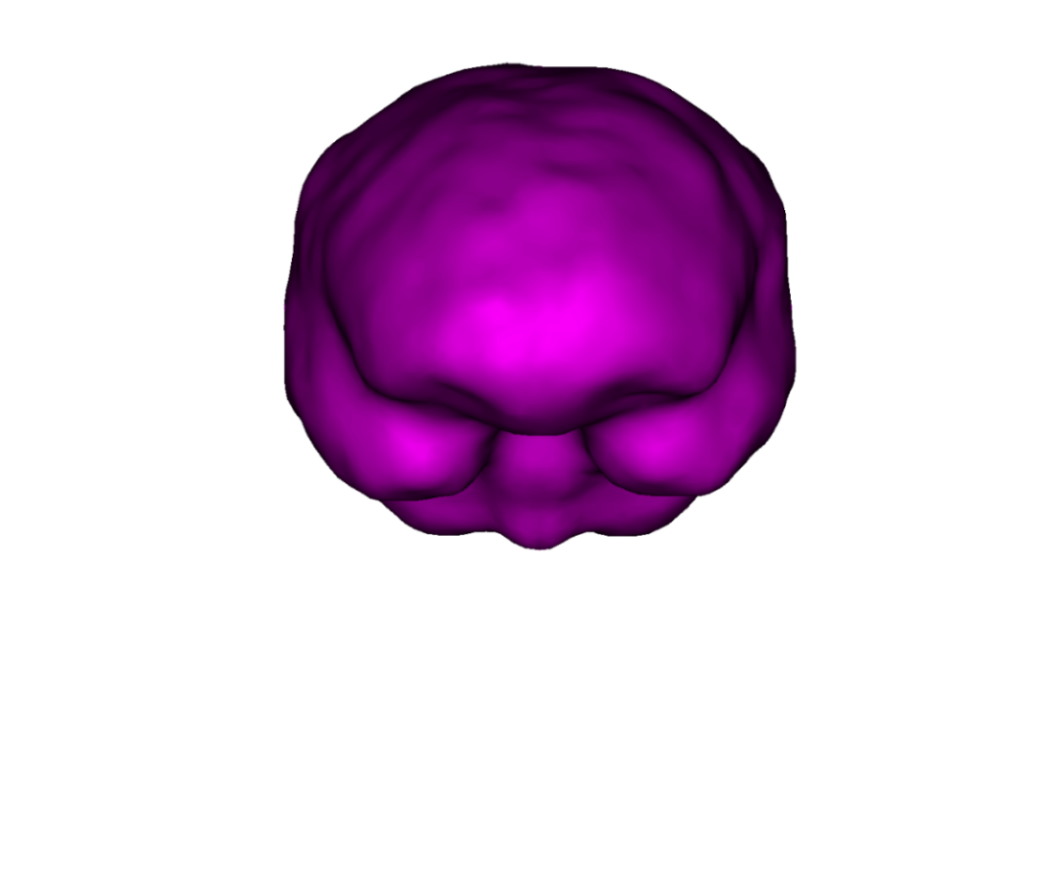
\includegraphics[width=5cm]{tete_couches_brain.png}\\
                            \parbox{5cm}{Surface extérieure au cortex}}
          \parbox[t]{5.5cm}{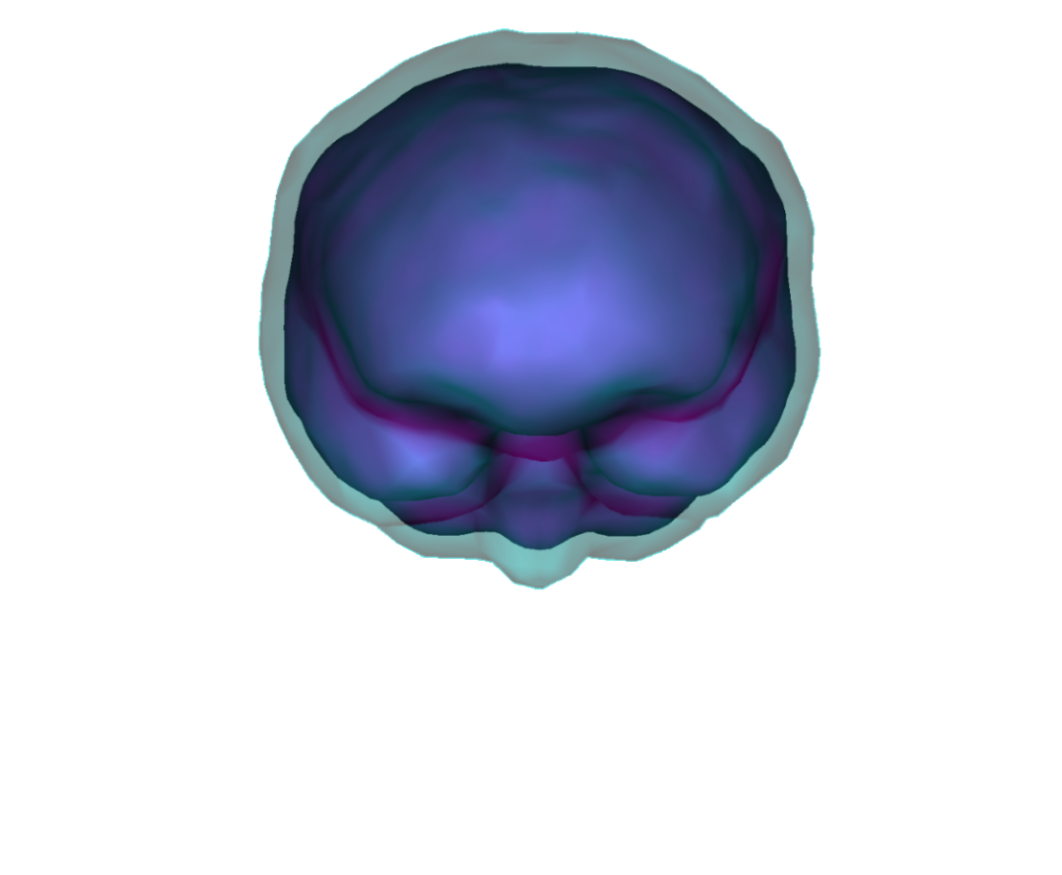
\includegraphics[width=5cm]{tete_couches_brainskull.png}\\\parbox{5cm}{Surface extérieure au crâne en bleu et surface extérieure au cortex en fushia}}
          \parbox[t]{5.5cm}{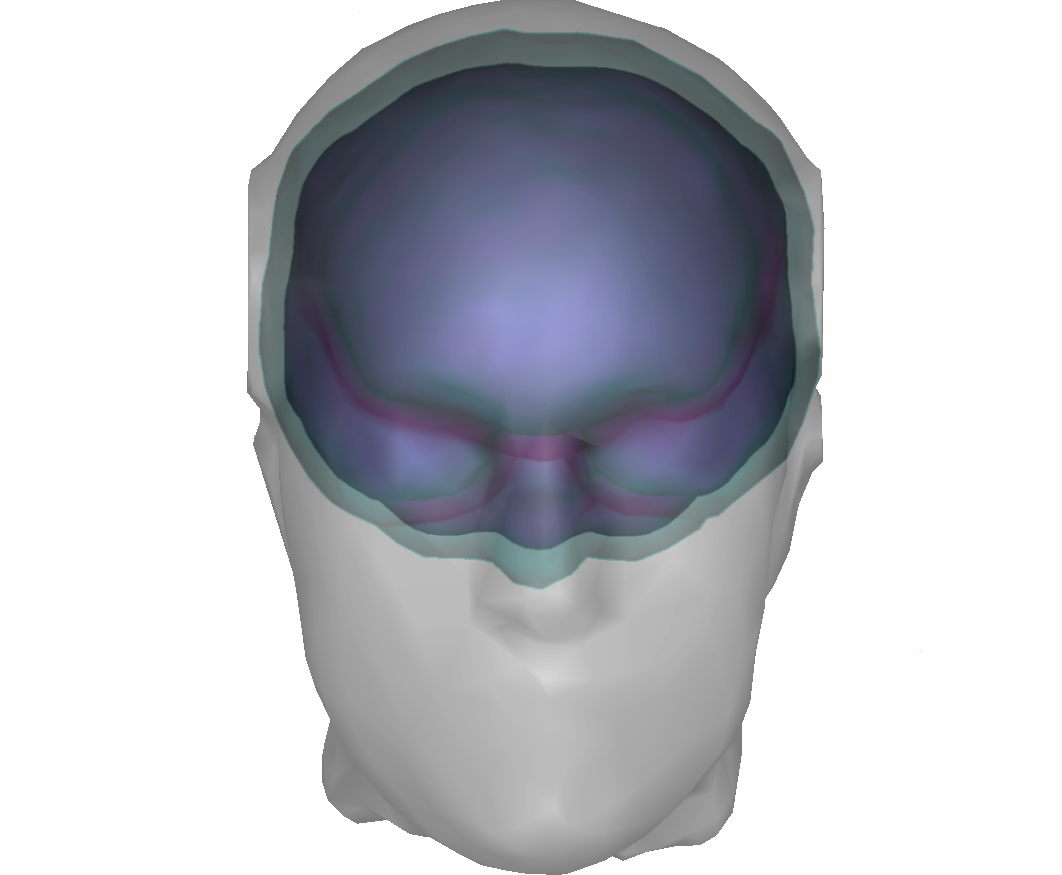
\includegraphics[width=5cm]{tete_couches_brainskullhead.png}\\
                            \parbox{5cm}{Exemple avec trois surfaces~:
                                  \begin{itemize}
                                       \item extérieure au scalp en gris
                                       \item extérieure au crâne en bleu
                                       \item extérieur au cortex en fushia
                                  \end{itemize}}
                            }
    }
}

\bigskip

\noindent
Dans le cas de sources distribuées, il faut un maillage de sources. Il s'agit généralement d'un maillage détaillé du cerveau. Nous conseillons un maillage de 30 000 à 35 000 points.

\begin{center}
    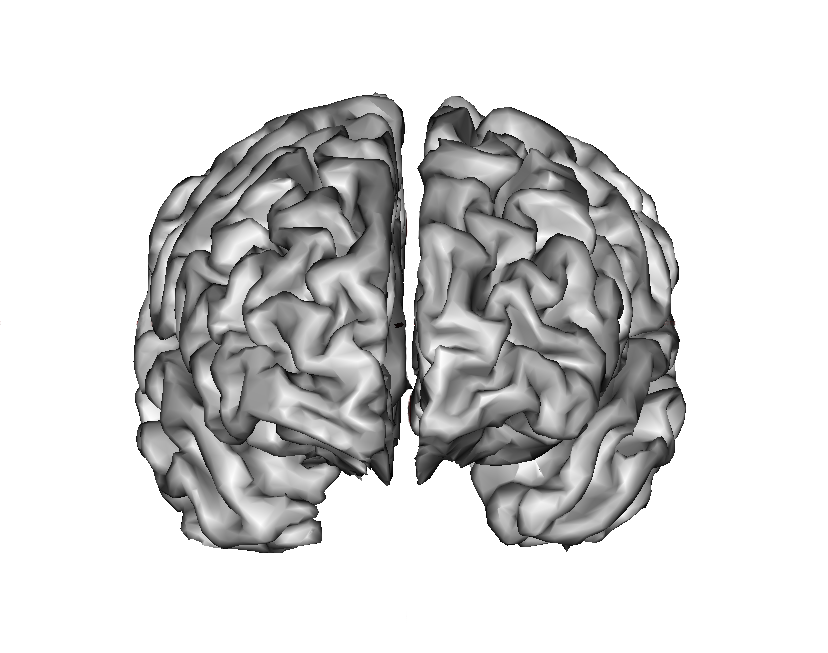
\includegraphics[height=9cm]{cortex.png}\\
    Maillage de sources
\end{center}

\noindent
\underline{Capteurs}~:
	Dans le cas de l'EEG, un fichier de description de la position des électrodes (ou patches) en coordonnées cartésiennes.
